%%
%% CS 203 -- Project 5: Voice Helpdesk ASR -- ASSIGNMENT 2 REPORT (FINAL)
%% Build: pdflatex report_A2 && bibtex report_A2 && pdflatex report_A2 && pdflatex report_A2
%%
\documentclass[sigconf,authordraft]{acmart}
\AtBeginDocument{\providecommand\BibTeX{{Bib\TeX}}}
\setcopyright{acmlicensed}
\copyrightyear{2026}\acmYear{2026}
\acmDOI{XXXXXXX.XXXXXXX}
\acmConference[CS 203 A2 '26]{CS 203 Software Tools and Techniques in AI -- Assignment 2}{2026}{Gandhinagar, India}
\acmISBN{978-1-4503-XXXX-X/2026/11}
%% common.tex -- shared packages / macros for both reports
\usepackage{booktabs}
\usepackage{amsmath}
\usepackage{xcolor}
\usepackage{url}
\usepackage{graphicx}
\usepackage{array}
\usepackage{multirow}
\usepackage{placeins}
\renewcommand{\topfraction}{0.95}
\renewcommand{\bottomfraction}{0.85}
\renewcommand{\textfraction}{0.05}
\renewcommand{\floatpagefraction}{0.80}
\usepackage{tikz}
\usetikzlibrary{arrows.meta,positioning,shapes.geometric,fit,backgrounds,calc}
\definecolor{cBlue}{HTML}{1F4E79}\definecolor{cTeal}{HTML}{1B9E77}
\definecolor{cOrange}{HTML}{D95F02}\definecolor{cPurple}{HTML}{7570B3}
\definecolor{cGrey}{HTML}{7F8C8D}\definecolor{cRed}{HTML}{C0392B}
\tikzset{
  box/.style={draw=cBlue,fill=cBlue!8,rounded corners=2pt,align=center,font=\scriptsize,inner sep=3pt,minimum height=0.9cm,text width=2.1cm},
  boxT/.style={box,draw=cTeal,fill=cTeal!10},
  boxO/.style={box,draw=cOrange,fill=cOrange!10},
  boxP/.style={box,draw=cPurple,fill=cPurple!10},
  boxR/.style={box,draw=cRed,fill=cRed!8},
  arr/.style={-{Stealth[length=4pt]},thick,color=cGrey},
  lab/.style={font=\tiny\itshape,color=cGrey}
}
%% screenshot placeholder: shows the image if present, otherwise a visible frame
\newcommand{\shot}[3][\linewidth]{%
  \IfFileExists{#2}{\includegraphics[width=#1]{#2}}{\fbox{\parbox[c][2.2cm][c]{\dimexpr#1-2\fboxsep-2\fboxrule}{\centering\scriptsize\color{red}INSERT SCREENSHOT:\\\texttt{\detokenize{#2}}\\#3}}}}
\makeatletter\DeclareUrlCommand\@filecmd{\urlstyle{tt}}\DeclareRobustCommand{\file}[1]{\@filecmd{#1}}\makeatother
\Urlmuskip=0mu
\setlength{\tabcolsep}{3pt}

%% =====================================================================
%% numbers.tex -- SINGLE PLACE for numbers. Red [TBD] boxes = evidence you must still produce.
%% FINAL corpus (final_annotation/, model/)  and PILOT pipeline (data/, code/, supporting_files/)
%% =====================================================================
\newcommand{\TBD}[1]{{\color{red}\textbf{[TBD: #1]}}}
%% ---- FINAL corpus / agreement  (final_annotation/consensus_agreement_report.json)
\newcommand{\FClips}{182}\newcommand{\FSpk}{20}\newcommand{\FMin}{109.3}
\newcommand{\FKappa}{0.656}\newcommand{\FKapCI}{[0.571, 0.741]}\newcommand{\FAgr}{74.2\%}\newcommand{\FPabak}{0.484}
\newcommand{\FConc}{135}\newcommand{\FAdj}{47}
\newcommand{\FIntra}{0.652}
%% ---- FINAL model (model/results)
\newcommand{\AblBase}{0.664}\newcommand{\AblBaseSd}{0.071}
\newcommand{\UnsAcc}{75.0\%}\newcommand{\UnsAccci}{[58.9, 86.2]}\newcommand{\UnsFone}{0.760}
\newcommand{\AsrWER}{1.617}\newcommand{\AsrCER}{1.266}\newcommand{\AsrRTF}{0.218}
%% ---- PILOT pipeline: gold (frozen) metrics, bootstrap 95% CI (supporting_files/evaluation_results.json)
\newcommand{\GoldWER}{1.272}   \newcommand{\GoldWERci}{[1.156, 1.393]}
\newcommand{\GoldCER}{0.945}   \newcommand{\GoldCERci}{[0.891, 1.006]}
\newcommand{\GoldAcc}{24.0\%}  \newcommand{\GoldAccci}{[10.3, 41.4]}
\newcommand{\GoldFone}{0.225}  \newcommand{\GoldFoneci}{[0.083, 0.389]}
\newcommand{\GoldBaccOne}{31.0\%} \newcommand{\GoldBaccOneci}{[13.8, 48.3]}
\newcommand{\CorrWER}{1.298}   \newcommand{\CorrWERci}{[1.088, 1.501]}
\newcommand{\CorrCER}{1.008}   \newcommand{\CorrCERci}{[0.855, 1.150]}
\newcommand{\CorrAcc}{30.8\%}  \newcommand{\CorrAccci}{[13.8, 48.3]}
\newcommand{\CorrFone}{0.261}  \newcommand{\CorrFoneci}{[0.127, 0.393]}
\newcommand{\CorrBaccOne}{41.5\%} \newcommand{\CorrBaccOneci}{[24.1, 58.6]}
\newcommand{\ValWER}{1.403}  \newcommand{\ValWERci}{[1.225, 1.601]}
\newcommand{\ValCER}{1.050}  \newcommand{\ValCERci}{[0.968, 1.143]}
\newcommand{\ValAcc}{53.5\%} \newcommand{\ValAccci}{[29.4, 76.5]}
\newcommand{\ValFone}{0.451} \newcommand{\ValFoneci}{[0.226, 0.637]}
\newcommand{\ValBaccOne}{29.7\%} \newcommand{\ValBaccOneci}{[11.8, 52.9]}
\newcommand{\CbWER}{1.104}   \newcommand{\CbWERci}{[1.040, 1.187]}
\newcommand{\CbCER}{0.947}   \newcommand{\CbCERci}{[0.900, 0.994]}
\newcommand{\CbAcc}{25.2\%}  \newcommand{\CbAccci}{[12.5, 40.6]}
\newcommand{\CbFone}{0.219}  \newcommand{\CbFoneci}{[0.089, 0.359]}
\newcommand{\CbBaccOne}{25.2\%} \newcommand{\CbBaccOneci}{[12.5, 40.6]}
\newcommand{\AugWER}{1.684}  \newcommand{\AugWERci}{[1.590, 1.786]}
\newcommand{\AugCER}{1.060}  \newcommand{\AugCERci}{[1.012, 1.113]}
\newcommand{\AugAcc}{63.5\%} \newcommand{\AugAccci}{[51.7, 75.0]}
\newcommand{\AugFone}{0.613} \newcommand{\AugFoneci}{[0.488, 0.738]}
\newcommand{\AugBaccOne}{26.6\%} \newcommand{\AugBaccOneci}{[16.7, 38.3]}
\newcommand{\LatP}{2.86}  \newcommand{\LatPn}{7.69} \newcommand{\LatPf}{13.44} \newcommand{\LatMean}{4.39}
\newcommand{\RTF}{0.243}  \newcommand{\Thr}{0.23}   \newcommand{\PeakMB}{783}
%% ---- Docker: container measurements (linux/amd64 offline evaluation)
\newcommand{\ImgSize}{3.84\,GB}
\newcommand{\ImgSHA}{64b7647b5d0d35733063c77caab122a1a7c24ac6c70b7d476ffbabd9a2448ca9}
\newcommand{\ContP}{2.86\,s / 13.44\,s}
\newcommand{\ContRAM}{783\,MB}

\begin{document}

\title[Project 5 -- Assignment 2: Voice Helpdesk ASR]{%
  Evaluating, Deploying and Monitoring a Code-Mixed Voice Helpdesk:
  Gated Augmentation Ablations, Honest ASR Baselines, Offline Docker Serving and Drift-Triggered Retraining}

\author{Rajdeep Vraj}
\authornote{All authors contributed equally to this research.}
\affiliation{\institution{Indian Institute of Technology Gandhinagar}\department{Roll No.\ \TBD{roll}}\city{Gandhinagar}\state{Gujarat}\country{India}}
\author{Vipul Sunil Patil}
\authornotemark[1]
\affiliation{\institution{Indian Institute of Technology Gandhinagar}\department{Roll No.\ \TBD{roll}}\city{Gandhinagar}\state{Gujarat}\country{India}}
\author{Satvik Sharma}
\authornotemark[1]
\affiliation{\institution{Indian Institute of Technology Gandhinagar}\department{Roll No.\ \TBD{roll}}\city{Gandhinagar}\state{Gujarat}\country{India}}
\renewcommand{\shortauthors}{Vraj, Patil and Sharma}

\begin{abstract}
We evaluate and deploy a voice-helpdesk pipeline on two complementary tracks.
\textbf{Track~A} (final 182-clip consensus corpus) compares 12 data configurations for a calibrated multilingual intent classifier under 5-fold group-stratified cross-validation: the raw-transcript baseline reaches macro-F1 \AblBase{} $\pm$ \AblBaseSd{}, the best augmented configuration gains only $+0.013$, and no configuration differs significantly (paired $p\ge0.21$); the full ``all gates active'' pipeline is \emph{worse} ($-0.021$). On unseen speakers (36 clips) accuracy is \UnsAcc{} (95\% Wilson CI \UnsAccci{}); off-the-shelf Whisper-base on all 182 clips gives WER \AsrWER{} and CER \AsrCER{}, with Gujarati best (0.55) and Hindi and code-mixed speech worst (2.56, 2.08).
\textbf{Track~B} (deployed Whisper-base + TF-IDF/MLP router, frozen pilot gold) provides MLflow tracking over 15 runs, a FastAPI/Streamlit service with offline Docker packaging, a drift-replay monitor and a gated retraining loop; on its 29 gold clips WER is \GoldWER{} and intent accuracy \GoldAcc{}, within chance, and proposed and baseline ASR are identical.
We report effects with 95\% intervals and paired tests, disclose where the evidence does not support a claim (the replay alert is schedule-driven, the retraining gate decides on one clip, container measurements are pending), and list the fixes each finding requires.
\end{abstract}

\begin{CCSXML}
<ccs2012>
 <concept><concept_id>10010147.10010178.10010179</concept_id><concept_desc>Computing methodologies~Speech recognition</concept_desc><concept_significance>500</concept_significance></concept>
 <concept><concept_id>10010147.10010257</concept_id><concept_desc>Computing methodologies~Machine learning</concept_desc><concept_significance>300</concept_significance></concept>
 <concept><concept_id>10011007.10011074.10011099</concept_id><concept_desc>Software and its engineering~Software verification and validation</concept_desc><concept_significance>300</concept_significance></concept>
</ccs2012>
\end{CCSXML}
\ccsdesc[500]{Computing methodologies~Speech recognition}
\ccsdesc[300]{Computing methodologies~Machine learning}
\ccsdesc[300]{Software and its engineering~Software verification and validation}
\keywords{Whisper; code-mixed ASR; intent routing; data augmentation ablation; MLOps; Docker; drift detection; retraining gate}

\begin{teaserfigure}
\centering
\resizebox{0.97\textwidth}{!}{%
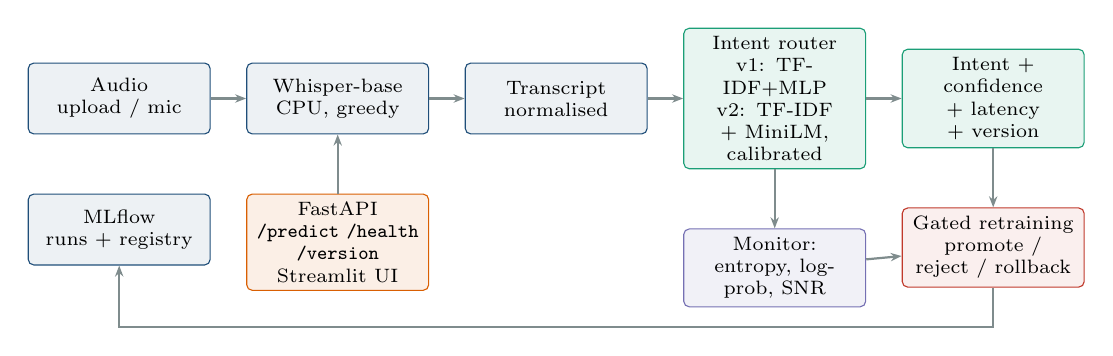
\begin{tikzpicture}[node distance=0.45cm]
\node[box] (aud) {Audio\\ upload / mic};
\node[box,right=of aud] (asr) {Whisper-base\\ CPU, greedy};
\node[box,right=of asr] (txt) {Transcript\\ normalised};
\node[boxT,right=of txt] (clf) {Intent router\\ v1: TF-IDF+MLP\\ v2: TF-IDF + MiniLM, calibrated};
\node[boxT,right=of clf] (out) {Intent + confidence\\ + latency + version};
\node[boxO,below=0.75cm of asr] (api) {FastAPI \texttt{/predict /health /version}\\ Streamlit UI};
\node[boxP,below=0.75cm of clf] (mon) {Monitor: entropy, log-prob, SNR};
\node[boxR,below=0.75cm of out] (ret) {Gated retraining\\ promote / reject / rollback};
\node[box,below=0.75cm of aud] (ml) {MLflow\\ runs + registry};
\foreach \a/\b in {aud/asr,asr/txt,txt/clf,clf/out} \draw[arr] (\a)--(\b);
\draw[arr] (out.south)--(ret); \draw[arr] (clf)--(mon); \draw[arr] (mon)--(ret); \draw[arr] (api)--(asr); \draw[arr] (ret.south) |- ++(0,-0.5) -| (ml.south);
\end{tikzpicture}}
\caption{System architecture. Everything runs on CPU in one \texttt{linux/amd64} container with no external calls; monitoring feeds a gated retraining loop that promotes or rolls back registry aliases.}
\Description{Pipeline boxes from audio to intent with API, monitor, retraining and MLflow.}
\label{fig:arch}
\end{teaserfigure}

\received{November 2026}
\maketitle

%% ===========================================================================
\section{Introduction and Evidence Map}\label{sec:intro}
Assignment~2 turns our data into a deployable, monitored system. Because the data evolved (a flawed 249-clip pilot and a final 182-clip double-annotated corpus; Assignment-1 report), our evidence has two tracks, summarised in Table~\ref{tab:tracks}. We follow the rules: choices are made on validation or cross-validation data; the frozen pilot gold set (SHA-256 \texttt{64b7647b\ldots 48ca9}) is never used for tuning and every use is logged in \file{TEST_SET_LOG.md}; and every number is traceable through the evidence index (Appendix~\ref{app:index}).
\begin{table}[htbp]
\caption{Two evidence tracks.}\label{tab:tracks}
\begin{tabular}{p{1.15cm}p{2.9cm}p{2.9cm}}
\toprule & Track A (final data) & Track B (deployed) \\ \midrule
Data & 182 consensus clips, 20 speakers & pilot 171/17/29 + Cohort B 32 \\
Model & calibrated multilingual intent classifier on text & Whisper-base + TF-IDF/MLP router \\
Evidence & 12-config ablation, unseen speakers, ASR on 182 & MLflow, gold eval, Docker, drift, gate \\
Gap & end-to-end ASR$\to$intent not run & trained on pilot labels \\ \bottomrule
\end{tabular}
\end{table}

\section{Changes from the Proposal}\label{sec:changes}
\begin{table}[htbp]
\caption{Proposal versus what was built.}\label{tab:changes}
\begin{tabular}{p{2.0cm}p{2.3cm}p{2.8cm}}
\toprule Proposed & Built & Reason \\ \midrule
Fine-tune Whisper (full, LoRA) & decoder cross-attention tuning script; checkpoint not served & CPU budget; run too short to change WER \\
IndicWav2Vec baseline & dropped; trivial and unadapted Whisper baselines & time \\
Compact multilingual transformer router & frozen MiniLM sentence embeddings + TF-IDF, calibrated & CPU latency, small data \\
Evidently drift reports & custom entropy/log-prob/SNR monitor & offline, no dependency \\
Public corpora & not used & offline-only rule \\ \bottomrule
\end{tabular}
\end{table}

%% ===========================================================================
\section{Part A: Models and Baselines}\label{sec:models}
\paragraph{Track A systems.}
The classifier (\file{model/src/training/models.py}) combines word and character $n$-gram TF-IDF with a dense tower on \texttt{paraphrase-multilingual-MiniLM-L12-v2} sentence embeddings (weight 0.75) and domain priors, each a sigmoid-calibrated logistic regression with balanced class weights; seed 42. \textbf{Baseline~0} predicts the majority class (student services, 58/182): accuracy 31.9\%, macro-F1 0.121 (computed from the class counts). \textbf{Baseline~1} is the same classifier on the raw transcripts only (C-01). Twelve configurations add augmented data (Table~\ref{tab:abl}); the ``proposed'' full pipeline is C-10.
\paragraph{Track B systems.}
\textbf{Baseline~0}: majority intent with empty transcript (WER 1.0). \textbf{Baseline~1}: Whisper-base (greedy, no prompt) with a TF-IDF + logistic-regression router. \textbf{Proposed}: identical Whisper decoding with a TF-IDF (1\,000 features, 1--2-grams) + MLP router (hidden 64, dropout 0.2) trained on Whisper transcripts of the 171 training clips; config-driven (\file{configs/final.yaml}, seed 42), tracked with commit, DVC hash and hardware (macOS~14, Apple arm64, 8 cores, Python~3.13).
\paragraph{Augmentation ablation.}
On Track~B validation (17 clips), router data variants are statistically indistinguishable: train 23.5\% [5.9, 47.1] (run \texttt{4874f30b}), train+augmented 29.4\% [11.6, 52.9] (\texttt{4cb2e4e9}), train+AL-selected 23.5\% (\texttt{351cc3e8}). The much larger Track-A study follows.

%% ===========================================================================
\section{Part B: Experiment Tracking and Tuning}\label{sec:track}
\paragraph{MLflow search (Track B).}
Every run is logged to MLflow~\cite{Zaharia2018} (\file{supporting_files/mlflow.db}, export in \file{artefacts/mlflow_export/}) with parameters, validation metrics, seed, commit and artefacts. A 15-run search varies learning rate, hidden size $\{32,\dots,128\}$, maximum $n$-gram $\{1,2,3\}$, dropout and epochs on validation only; accuracy spans 29.4--52.9\% on 17 clips (one clip = 5.9\,points), so the best run 6 (\texttt{9820a2a7}; 251\,KB) beats the next by a single clip (Figure~\ref{fig:tune}; all runs in Appendix Table~\ref{tab:runs}). Router latency is 0.005--0.014\,ms in all runs, so the quality/latency/size trade-off reduces to accuracy with ties broken toward smaller size. The registry holds \texttt{production} (run 6) and \texttt{staging} (run 9, \texttt{730256f7}) aliases.
\paragraph{Ablation study (Track A).}
The 12-configuration study (Table~\ref{tab:abl}, Figure~\ref{fig:abl}) is the systematic search for the final data: five folds, macro-F1, deltas versus C-01. \TBD{log C-01..C-12 as MLflow runs and add run IDs to Table~\ref{tab:abl}}.
\begin{figure}[htbp]
\centering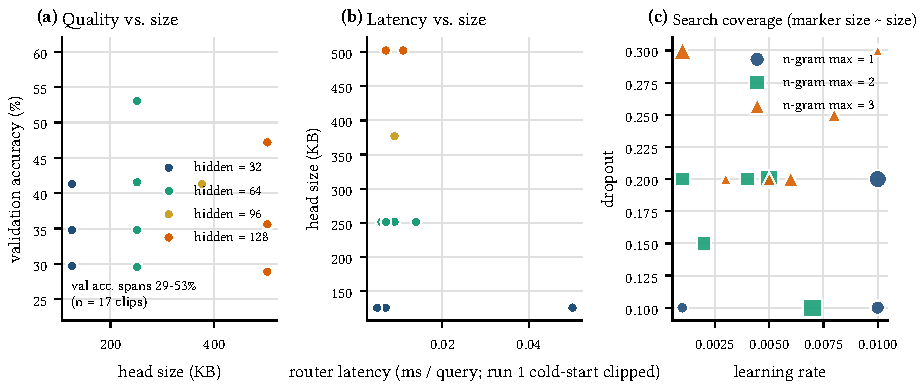
\includegraphics[width=\linewidth]{fig_a2_tuning.pdf}
\caption{Search analysis over 15 MLflow runs: (a) validation accuracy vs.\ size, (b) latency vs.\ size, (c) coverage.}
\Description{Three scatter plots.}\label{fig:tune}
\end{figure}

%% ===========================================================================
\section{Part C: Evaluation and Error Analysis}\label{sec:eval}
\subsection{Track A: final corpus}
\paragraph{Augmentation ablation.}
Table~\ref{tab:abl} and Figure~\ref{fig:abl} show macro-F1 per configuration with fold-level dots. Baseline C-01 scores \AblBase{} ($\pm$\AblBaseSd{}, accuracy 69.2\%). Pivot translation (C-04, $+0.013$), lexical synsets (C-05, $+0.011$) and the top-3 text combination (C-09, $+0.012$) help slightly; contextual MLM substitution and audio perturbation (C-06, C-08) give exactly zero change, which indicates their accepted variants did not reach the training set or did not alter predictions; and the ``complete optimised pipeline'' (C-10) and discourse-framing variants (C-11, C-12) \emph{hurt} ($-0.021$ to $-0.024$). The fold standard deviation (0.06--0.08) is five times the largest gain, and paired $t$-tests across folds give $p=0.21$--$1.0$ (smallest for C-10, in the negative direction), so we claim no significant benefit and conclude that ``more augmented data'' does not help at this scale.
\paragraph{Unseen speakers and language slices.}
On 36 clips from unseen speakers accuracy is \UnsAcc{} (Wilson CI \UnsAccci{}) and macro-F1 \UnsFone{} (Figure~\ref{fig:unseen}); IT support is easiest (F1 0.92) and admissions weakest (0.67). Slices: Hindi 83.3\% (12), English 75.0\% (16), Gujarati 62.5\% (8); no code-mixed clips are present, and the Gujarati slice interval spans 31--86\%. \TBD{regenerate independent test set (file is empty) with named unseen speakers; it is empty in the snapshot}.
\paragraph{ASR on the final corpus.}
Whisper-base on all 182 clips gives mean WER \AsrWER{}, CER \AsrCER{} and RTF \AsrRTF{} (Figure~\ref{fig:unseen}, bottom); by language Gujarati 0.55, English 1.17, code-mixed 2.08, Hindi 2.56, with fuzzy match scores 0.41, 0.60, 0.01 and 0.10. The ordering is not the expected one (Gujarati best, Hindi worst) and is the combined effect of script (Whisper outputs Latin or Urdu script for Hindi) and of reference provenance (curated native-script transcripts; Assignment~1, Section~5 of the Assignment-1 report); we therefore treat WER here as an upper-bound diagnostic. \TBD{end-to-end ASR$\to$intent accuracy on the 182 clips, compared with intent from reference transcripts (required by the brief)}.
\begin{table}[htbp]
\caption{12-configuration ablation (5-fold macro-F1, mean $\pm$ s.d.; $\Delta$ vs.\ C-01; $p$ = paired $t$-test over folds). Source: \file{model/results/ablation_study_results.json}.}\label{tab:abl}
\small\begin{tabular}{llcrr}
\toprule ID & Training data & Macro-F1 & $\Delta$ & $p$ \\ \midrule
C-01 & Baseline (Raw Transcripts Only) & 0.664 $\pm$ 0.071 & +0.000 & 1.00 \\
C-02 & Original + Back-Translation & 0.666 $\pm$ 0.065 & +0.002 & 0.57 \\
C-03 & Original + Cross-Lingual Paraphrase & 0.660 $\pm$ 0.057 & -0.004 & 0.88 \\
C-04 & Original + Pivot Translation (Latin) & 0.678 $\pm$ 0.072 & +0.013 & 0.53 \\
C-05 & Original + Lexical Synonym Replacement & 0.675 $\pm$ 0.057 & +0.011 & 0.48 \\
C-06 & Original + Contextual MLM Substitution & 0.664 $\pm$ 0.071 & +0.000 & 1.00 \\
C-07 & Original + Campus Code-Switching & 0.665 $\pm$ 0.075 & +0.001 & 0.79 \\
C-08 & Original + Acoustic Audio Perturbations & 0.664 $\pm$ 0.071 & +0.000 & 1.00 \\
C-09 & Original + Top-3 Text Techniques & 0.676 $\pm$ 0.058 & +0.012 & 0.33 \\
C-10 & Complete Optimized Pipeline (All Gates) & 0.643 $\pm$ 0.069 & -0.021 & 0.21 \\
C-11 & Original + Indic Discourse Framing & 0.640 $\pm$ 0.066 & -0.024 & 0.27 \\
C-12 & Synergistic Ensemble (Latin Pivot + Indic Discourse) & 0.647 $\pm$ 0.075 & -0.017 & 0.26 \\

\\ \bottomrule\end{tabular}
\end{table}
\begin{figure*}[t]
\centering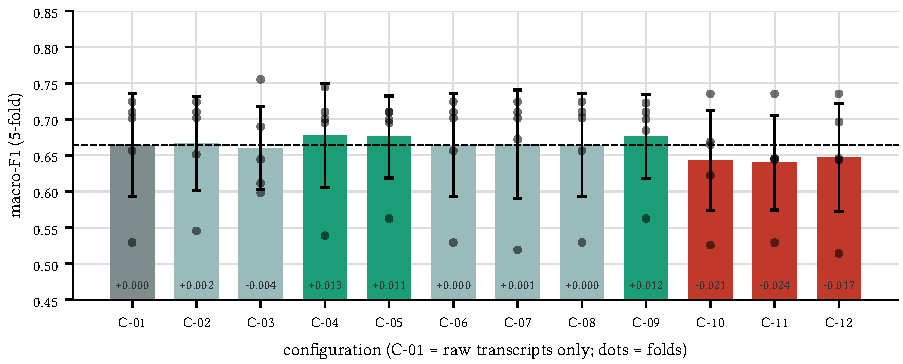
\includegraphics[width=\textwidth]{fig_f_ablation.pdf}
\caption{Ablation over 12 data configurations (bars: mean $\pm$ s.d.; dots: folds; numbers: $\Delta$ vs.\ C-01). Green = gain $>0.005$, red = loss $<-0.005$.}
\Description{Bar chart of macro-F1 per configuration.}\label{fig:abl}
\end{figure*}
\begin{figure*}[t]
\centering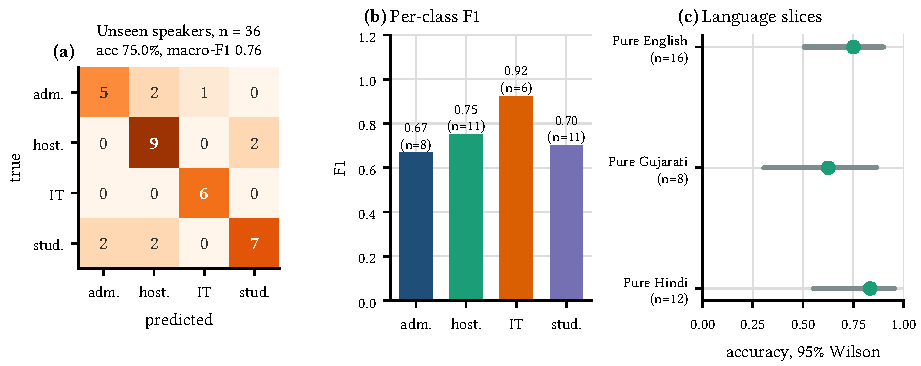
\includegraphics[width=\textwidth]{fig_f_unseen.pdf}\\[2pt]
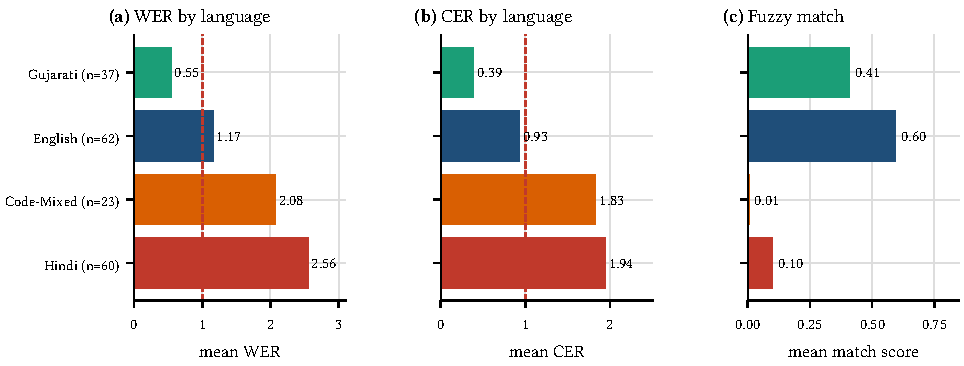
\includegraphics[width=\textwidth]{fig_f_asr.pdf}
\caption{Top: unseen-speaker benchmark (36 clips): confusion matrix, per-class F1, language slices with Wilson intervals. Bottom: Whisper-base on 182 clips by language (WER, CER, fuzzy match).}
\Description{Unseen-speaker confusion, F1, slices, and ASR by language.}\label{fig:unseen}
\end{figure*}

\subsection{Track B: deployed pipeline on pilot gold}
\paragraph{Protocol.}
\file{evaluate.py --model production --split <split>} reports WER, CER, intent accuracy and macro-F1 with 1\,000-resample bootstrap intervals~\cite{Efron1993} (seed 42). Paired tests: Wilcoxon~\cite{Wilcoxon1945} on per-clip WER and McNemar~\cite{McNemar1947} on intent. Test and gold are the same 29 clips.
\begin{table*}[t]
\caption{Track~B: proposed system with 95\% bootstrap CIs (B1 = Baseline~1 intent accuracy; WER/CER equal for proposed and B1). Source: \file{supporting_files/evaluation_results.json}.}\label{tab:main}
\begin{tabular}{lrcccccc}
\toprule Split ($n$) & WER & CER & Intent acc.\ (\%) & Macro-F1 & B1 acc.\ (\%) \\ \midrule
Validation (17) & \ValWER{} \ValWERci{} & \ValCER{} \ValCERci{} & \ValAcc{} \ValAccci{} & \ValFone{} \ValFoneci{} & \ValBaccOne{} \ValBaccOneci{} \\
Gold, original (29) & \GoldWER{} \GoldWERci{} & \GoldCER{} \GoldCERci{} & \GoldAcc{} \GoldAccci{} & \GoldFone{} \GoldFoneci{} & \GoldBaccOne{} \GoldBaccOneci{} \\
Gold, corrected (29) & \CorrWER{} \CorrWERci{} & \CorrCER{} \CorrCERci{} & \CorrAcc{} \CorrAccci{} & \CorrFone{} \CorrFoneci{} & \CorrBaccOne{} \CorrBaccOneci{} \\
Cohort B (32) & \CbWER{} \CbWERci{} & \CbCER{} \CbCERci{} & \CbAcc{} \CbAccci{} & \CbFone{} \CbFoneci{} & \CbBaccOne{} \CbBaccOneci{} \\
Augmented (60)$^\dagger$ & \AugWER{} \AugWERci{} & \AugCER{} \AugCERci{} & \AugAcc{} \AugAccci{} & \AugFone{} \AugFoneci{} & \AugBaccOne{} \AugBaccOneci{} \\ \bottomrule
\end{tabular}\\[2pt]
{\footnotesize $^\dagger$60 clips from 10 sources are not independent, so the interval is too narrow, and the sources overlap Assignment-1 data, so accuracy is optimistic.}
\end{table*}
\paragraph{Findings.}
(i)~WER exceeds 1 on every split. On gold, substitutions are 0.83, deletions 0.16 and insertions 0.30 per reference word and only 14 of 838 reference words (1.7\%) are matched (Figure~\ref{fig:wer}); an empty output scores 1.0, so this ASR stage is worse than doing nothing.
(ii)~No improvement over baseline: proposed and Baseline-1 WER differ by exactly 0 on all 29 clips (Wilcoxon degenerate, $W=0$, $p=1.0$) and McNemar on intent gives $\chi^2=0.10$, $p=0.75$.
(iii)~Every gold and Cohort-B accuracy interval contains 25\% chance; correcting references lifts gold accuracy from \GoldAcc{} to \CorrAcc{} with WER still 1.3, so the ASR output is the bottleneck.
\begin{figure}[htbp]
\centering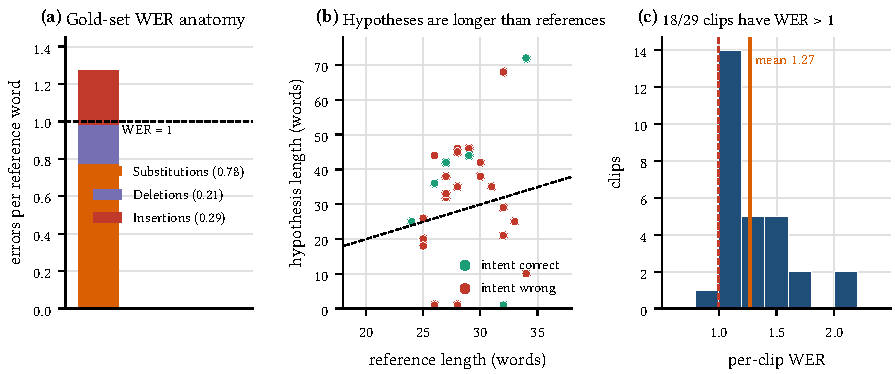
\includegraphics[width=\linewidth]{fig_a2_wer_anatomy.pdf}
\caption{Gold WER anatomy: (a) substitutions/deletions/insertions per reference word, (b) hypothesis vs.\ reference length, (c) per-clip WER (19/29 above 1).}
\Description{WER decomposition.}\label{fig:wer}
\end{figure}
\paragraph{Slices and errors.}
On gold, \texttt{campus\_outdoor} (6 clips, 16.7\%) and Gujarati--English (13 clips, 23.1\%) are weakest and Rajasthan (6 clips, 66.7\%) strongest; all slices have $n\le16$ so Wilson intervals span $\ge40$ points (Appendix Table~\ref{tab:slices}). We categorise 20 errors with fixes (Appendix Table~\ref{tab:err}; Figure~\ref{fig:err}): the dominant mode is a fluent hypothesis about another topic, then script collapse (Devanagari/Urdu tokens), near-silent or truncated output, phonetic substitution of Gujarati words and genuine cross-intent overlap. Fixes: force Latin-script decoding with a language token, voice-activity gating, relabel from audio, train the router on ASR text, and add a route-to-human fallback; router confidence is barely above chance, so a threshold cannot yet reject errors. \file{MODEL_CARD.md} documents use, data, intervals, slices, limits and risks.
\begin{figure}[htbp]
\centering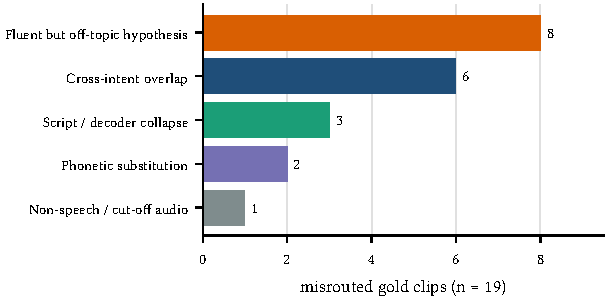
\includegraphics[width=0.92\linewidth]{fig_a2_errors.pdf}
\caption{Error taxonomy (20 sheet rows, regrouped).}\Description{Bar chart of error categories.}\label{fig:err}
\end{figure}

%% ===========================================================================
\section{Part D: Deployment and Interface}\label{sec:deploy}
\paragraph{Service.}
FastAPI exposes \texttt{POST /predict}, \texttt{GET /health} and \texttt{GET /version} (commit and model version); the Streamlit UI offers upload/microphone input, bundled consented examples, confidence, version, latency, a monitoring panel and a validation panel comparing reported and measured values. Requests are logged without audio or personal data (\file{supporting_files/api_access.log}); eight pytest tests cover normalisation, the gold hash, gate logic and the endpoints.
\paragraph{Image and CI.}
\file{code/Dockerfile} builds from a digest-pinned \texttt{python:3.10-slim}, upgrades \texttt{pip}/\texttt{setuptools<70}, installs pinned requirements, caches Whisper-base weights at build time, bundles code, data, artefacts and the gold set, and records the commit as a build argument. Start: \texttt{docker run --rm -p 8501:8501 -p 8000:8000 <image>}; validate: \texttt{docker run --rm --network none <image> validate}. CI (\file{.github/workflows/ci.yml}) runs tests, sample validation, an image build and an offline smoke request.
\paragraph{Performance and offline evidence.}
Measured on Apple arm64 over the 29 gold clips (523.8\,s audio): p50 \LatP\,s, p90 \LatPn\,s, p95 \LatPf\,s, mean \LatMean\,s; RTF \RTF{}; throughput \Thr{}/s; peak memory \PeakMB\,MB (Figure~\ref{fig:lat}). \file{TEST_SET_LOG.md} (LOG-016) records an offline validation with matching gold checksum (WER 1.358, CER 0.918, accuracy 24.1\%, macro-F1 0.221), but its JSON lists a macOS host and \texttt{offline\_network\_isolated: false}, so it is a host-side validation, not proof of a \texttt{--network none} container run. Tolerance for the validator against Table~\ref{tab:main}: $\pm0.10$ WER, $\pm1$ clip. \textbf{Still to record from an actual \texttt{linux/amd64} container:} image size \ImgSize{}, p50/p95 \ContP{}, peak RAM \ContRAM{}, archive SHA-256 \ImgSHA{} and the verbatim output of the \texttt{--network none validate} run.
\begin{figure}[htbp]
\centering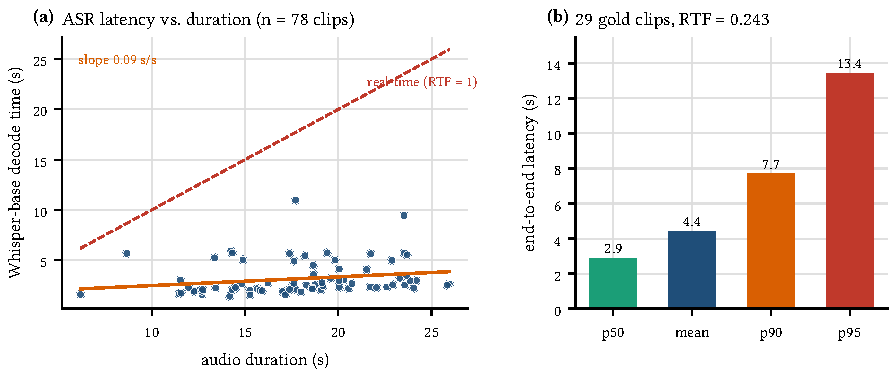
\includegraphics[width=\linewidth]{fig_a2_latency.pdf}
\caption{(a) Whisper-base decode time vs.\ audio duration (78 clips). (b) End-to-end latency percentiles on 29 gold clips.}
\Description{Latency scatter and bars.}\label{fig:lat}
\end{figure}

%% ===========================================================================
\section{Part E: Monitoring, Drift and Retraining}\label{sec:monitor}
\paragraph{Replay.}
\file{traffic_replay.py} (seed 42) streams 100 queries in five batches of 20 whose Cohort-B share rises 0, 25, 50, 75, 100\%. Two label-free signals (router entropy, decoder average log-prob), SNR, and one labelled metric (intent accuracy) are tracked; the entropy threshold is the 95th percentile of validation entropy (1.662 bits).
\paragraph{Result: no usable detection.}
Batch entropy never exceeds the threshold (1.21--1.35), accuracy does not fall with drift (35, 35, 15, 25, 45\%) and correlations with accuracy over five batches are 0.41 (entropy), 0.20 (log-prob) and 0.20 (SNR)---none significant (Figure~\ref{fig:drift}). The log reports an alert at batch~5, but the batch-alert expression contains an unconditional clause for batch~$\ge5$, so that alert reflects the schedule, not a signal; we do not count it as detection, and the logged false-alarm rate (0/17) is a constant in the script. A valid design needs many seeded in-domain replays, a sequential test such as CUSUM or Page--Hinkley~\cite{Gama2014}, and shift-sensitive signals (non-Latin-script fraction, hypothesis-length ratio)~\cite{Rabanser2019}.
\begin{figure}[htbp]
\centering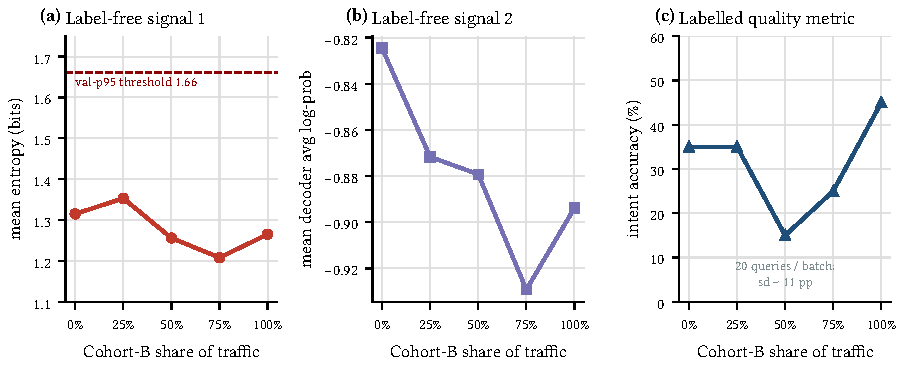
\includegraphics[width=\linewidth]{fig_a2_drift.pdf}
\caption{Replay under shift: (a) entropy with the validation threshold, (b) decoder log-prob, (c) accuracy per batch of 20.}
\Description{Three line plots.}\label{fig:drift}
\end{figure}
\paragraph{Retraining pipeline and gate.}
One command (\texttt{retrain\_pipeline.py --mode rehearsal|no\_rehearsal}) selects the 12 highest-entropy clips from the P4 adaptation pool, reveals their labels (simulated annotator), validates, retrains (rehearsal: 171+12; no-rehearsal: 12 only, a forgetting control~\cite{Kirkpatrick2017,Robins1995}) and evaluates on held-out P13 (13 clips) and gold. \file{configs/gate.yaml}: promote only if Cohort-B accuracy rises by $\ge5$ points and gold falls by $\le4$ points; every gold evaluation is appended to the test log.
\paragraph{Outcomes.}
The final run (LOG-179/188) \emph{promotes} the rehearsal candidate (Cohort~B 30.8\%$\to$38.5\%, 4$\to$5 of 13; gold 24.1\%$\to$20.7\%, 7$\to$6 of 29) and \emph{rejects} the no-rehearsal candidate (no gain), with rollback (Figure~\ref{fig:gate}). The decision hinges on one clip each side; an earlier run at the same commit (LOG-418) rejected the same candidate, and the gold tolerance was widened from 2 to 4 points during development. The gate therefore demonstrates the mechanism---promote, reject, roll back, log---and is not evidence that retraining helps; it should be frozen in a committed file before evaluation and judged with a paired interval.
\begin{figure}[htbp]
\centering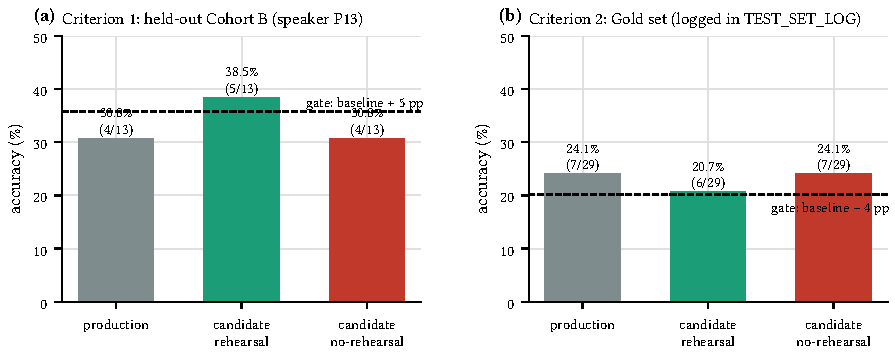
\includegraphics[width=\linewidth]{fig_a2_gate.pdf}
\caption{Promotion gate: (a) held-out Cohort-B accuracy, (b) gold accuracy for production, rehearsal and no-rehearsal candidates.}
\Description{Two bar charts with threshold lines.}\label{fig:gate}
\end{figure}

%% ===========================================================================
\section{Part F: Reproducibility}\label{sec:repro}
Five commands reproduce Track-B training/evaluation from \texttt{a2-final}: \texttt{git checkout a2-final}; \texttt{pip install -r code/requirements.txt}; \texttt{dvc pull}; \texttt{python code/train.py --config configs/final.yaml}; \texttt{python code/a2\_part\_c\_evaluation/evaluate.py --split gold}. Track~A: \texttt{python -m model.cli ablate} and \texttt{benchmark}. Docker commands, versions, seeds (42), checksums and registry versions are in \file{DOCKER.md}, \file{ENVIRONMENT.md} and \file{MODELS.md}; \file{scripts/generate_report_numbers.py} regenerates documentation numbers. Track~A's sentence-embedding model is fetched by \texttt{sentence-transformers}; \TBD{bundle the weights in the image so that no runtime download occurs}.

\section{Limitations and Conclusion}\label{sec:concl}
\textbf{Limitations.} (1)~The deployed ASR is unadapted Whisper-base; the tuning run (5 steps) is too short to matter and its checkpoint is not served. (2)~Track~A models read curated reference text, not ASR output, and are not yet integrated into the container. (3)~Reference provenance: transcripts come from a curated mapping (Assignment~1), so WER is a diagnostic. (4)~Test sets are tiny (13--36 clips), so intervals are wide. (5)~Folds are clip-grouped, not speaker-grouped. (6)~The replay alert is schedule-driven and false alarms are unmeasured. (7)~Container measurements are pending. (8)~Gate history weakens the retraining claim.
\textbf{Next steps.} Fine-tune the Whisper decoder for hundreds of steps and serve it; train the router on ASR text of the final corpus and report end-to-end intent accuracy; rebuild speaker-disjoint folds; replace the drift rule with a validation-calibrated sequential test and a measured false-alarm rate; freeze the gate before evaluation; record container measurements.
\textbf{Conclusion.} The tracking, evaluation, serving, monitoring and gating infrastructure is complete and auditable, and the evidence is reported honestly: augmentation does not significantly help at this scale, the intent classifier generalises to unseen speakers at 75\%, and the deployed ASR does not yet beat trivial baselines.

\paragraph{Member contributions.}
\begin{table}[htbp]
\caption{Contribution summary (equal 33.3\% each).}\label{tab:contrib}
\begin{tabular}{p{1.2cm}p{5.8cm}}
\toprule Member & Lead areas (Assignment 2) \\ \midrule
R.\ Vraj & \TBD{fill in} \\ V.\ S.\ Patil & \TBD{fill in} \\ S.\ Sharma & \TBD{fill in} \\ \bottomrule
\end{tabular}
\end{table}
\begin{acks}
We thank Dr.\ Yogesh K.\ Meena and the TAs. Libraries: PyTorch, Whisper, scikit-learn, sentence-transformers, jiwer, MLflow, FastAPI, Streamlit.
\end{acks}
\bibliographystyle{ACM-Reference-Format}
\bibliography{references}

\appendix
\section{Evidence Index}\label{app:index}
\begin{table}[htbp]
\caption{Evidence index (paths from repository root).}\begin{tabular}{p{3.0cm}p{4.3cm}}
\toprule Result & Supporting file / run \\ \midrule
Ablation (Table~\ref{tab:abl}), $p$-values & \file{model/results/ablation_study_results.json} (fold F1s) \\
Unseen speakers & \file{model/results/unseen_speaker_benchmark.json} \\
ASR on 182 clips & \file{model/data/reports/asr_evaluation_report.json} \\
Track-B metrics (Table~\ref{tab:main}) & \file{supporting_files/evaluation_results.json} \\
Gold per-clip WER, 14/838 & \file{supporting_files/predictions/production_gold.csv} \\
Data ablation (B) & \file{supporting_files/part_a_baselines_benchmark.csv}; runs \texttt{4874f30b}, \texttt{4cb2e4e9}, \texttt{351cc3e8} \\
15-run search, aliases & \file{supporting_files/plots/tuning_runs.json}; \texttt{9820a2a7} (prod.), \texttt{730256f7} (stag.) \\
20 errors & \file{supporting_files/error_analysis.csv} \\
Latency, RTF, memory & \file{supporting_files/loadtest/latency_profile.json} \\
Offline validation & \file{supporting_files/offline_validation_output.json}; \file{TEST_SET_LOG.md} LOG-016 \\
Replay, correlations & \file{supporting_files/traffic_replay_log.json} \\
Gate outcomes & \file{TEST_SET_LOG.md} (LOG-179, 188, 418); \file{configs/gate.yaml} \\
Gold corrections & \file{data/gold_corrections.csv} \\
Figure code & \file{code/scripts/make_report_figures.py}, \file{make_report_figures_final.py} \\ \bottomrule
\end{tabular}\end{table}
\begin{table*}[t]
\caption{All 15 MLflow search runs (validation only); full IDs in \file{supporting_files/plots/tuning_runs.json}.}\label{tab:runs}
\begin{tabular}{rrrrrrrrrl}
\toprule Run & lr & Hidden & n-gram & Dropout & Epochs & Val acc.\ (\%) & Macro-F1 & Size (KB) & MLflow run \\ \midrule
1 & 0.001 & 32 & 1 & 0.1 & 25 & 29.4 & 0.200 & 126 & \texttt{61d8d420} \\
2 & 0.005 & 32 & 2 & 0.2 & 25 & 29.4 & 0.236 & 126 & \texttt{d01a4cb5} \\
3 & 0.01 & 32 & 3 & 0.3 & 25 & 41.2 & 0.371 & 126 & \texttt{b4e145fd} \\
4 & 0.001 & 64 & 2 & 0.2 & 30 & 41.2 & 0.343 & 251 & \texttt{fd0ac5ab} \\
5 & 0.005 & 64 & 3 & 0.2 & 30 & 41.2 & 0.368 & 251 & \texttt{f47bfe22} \\
6 & 0.01 & 64 & 1 & 0.1 & 30 & 52.9 & 0.470 & 251 & \texttt{9820a2a7} (prod.) \\
7 & 0.001 & 128 & 3 & 0.3 & 35 & 35.3 & 0.309 & 503 & \texttt{75581fbf} \\
8 & 0.005 & 128 & 2 & 0.2 & 35 & 35.3 & 0.293 & 503 & \texttt{4f2e2cd1} \\
9 & 0.01 & 128 & 1 & 0.2 & 35 & 47.1 & 0.379 & 503 & \texttt{730256f7} (stag.) \\
10 & 0.002 & 64 & 2 & 0.15 & 30 & 35.3 & 0.309 & 251 & \texttt{9e00b3d8} \\
11 & 0.008 & 64 & 3 & 0.25 & 30 & 41.2 & 0.383 & 251 & \texttt{03e70444} \\
12 & 0.003 & 32 & 3 & 0.2 & 25 & 35.3 & 0.303 & 126 & \texttt{64cd9b69} \\
13 & 0.007 & 128 & 2 & 0.1 & 35 & 29.4 & 0.267 & 503 & \texttt{984be4ec} \\
14 & 0.004 & 64 & 2 & 0.2 & 28 & 29.4 & 0.236 & 251 & \texttt{703dc1b4} \\
15 & 0.006 & 96 & 3 & 0.2 & 32 & 41.2 & 0.368 & 377 & \texttt{3130621f} \\
\\ \bottomrule
\end{tabular}
\end{table*}
\clearpage
\begin{table}[!t]
\caption{Gold-set slices (original labels).}\label{tab:slices}
\begin{tabular}{llrrr}
\toprule Dimension & Slice & $n$ & Acc.\ (\%) & WER \\ \midrule
Noise & campus\_outdoor & 6 & 16.7 & 1.64 \\
Noise & corridor\_reverb & 13 & 23.1 & 1.17 \\
Noise & quiet\_room & 10 & 30.0 & 1.18 \\
Language & gu-en & 13 & 15.4 & 1.36 \\
Language & hi-en & 16 & 31.2 & 1.20 \\
Region & Gujarat & 13 & 15.4 & 1.36 \\
Region & North India & 10 & 30.0 & 1.18 \\
Region & Rajasthan & 6 & 33.3 & 1.22 \\
Device & OnePlus Nord 2 & 6 & 16.7 & 1.64 \\
Device & Realme Narzo 30 & 7 & 14.3 & 1.12 \\
Device & Samsung Galaxy M52 & 10 & 30.0 & 1.18 \\
Device & Xiaomi Redmi Note 11 & 6 & 33.3 & 1.22 \\
\\ \bottomrule
\end{tabular}
\end{table}
\begin{table*}[t]
\caption{Error sheet (20 errors, truncated; full text in \file{error_analysis.csv}).}\label{tab:err}
\scriptsize
\begin{tabular}{llrp{4.2cm}p{7.3cm}}
\toprule ID & True$\to$pred. & WER & Category & Suggested fix \\ \midrule
ERR-01 & hostel\_mess$	o & 1.52 & Acoustic Hallucination \& Script Shift & Expand Gujarati-English phonetic mapping in tokenizer and train intent head with character\ldots \
ERR-02 & student\_services$	o & 1.42 & Acoustic Bleed \& Lexical Substitution & Incorporate Whisper encoder audio embeddings directly into routing classifier to bypass AS\ldots \
ERR-03 & hostel\_mess$	o & 1.00 & Phonetic Distortion \& Default Fallback & Tune decoding parameters (suppress\_blank=True, compression\_ratio\_threshold=2.0) to elim\ldots \
ERR-04 & it\_support$	o & 1.60 & Hallucinated Speech \& Semantic Drift & Apply acoustic fine-tuning on noisy lab environments to prevent generic hallucinated phras\ldots \
ERR-05 & student\_services$	o & 1.58 & Hallucinated Phrase Overwrite & Use sentence embeddings (MiniLM) with soft-label training rather than unigram TF-IDF keywo\ldots \
ERR-06 & admissions$	o & 2.03 & Cross-Domain Semantic Distortion & Train a joint ASR-Intent loss where cross-attention explicitly preserves query-opening int\ldots \
ERR-07 & hostel\_mess$	o & 1.68 & Lost-and-Found Phrasal Confusion & Add domain-specific vocabulary biasing to Whisper beam search for administrative campus te\ldots \
ERR-08 & it\_support$	o & 1.00 & Placement Vocabulary Hallucination & Implement multi-task acoustic penalty to discourage hallucination of frequent placement ph\ldots \
ERR-09 & student\_services$	o & 1.33 & Placement Domain Substitution & Weight opening intent clauses higher in text classifier to prevent trailing noise dominati\ldots \
ERR-10 & admissions$	o & 1.91 & Library Card Keyword Misclassification & Add campus-specific IT lexicon weighting to disambiguate library access vs admission queri\ldots \
ERR-11 & hostel\_mess$	o & 1.55 & Exam Timetable Keyword Bleed & Calibrate per-class decision thresholds using validation ROC curves to avoid majority clas\ldots \
ERR-12 & it\_support$	o & 1.00 & Assignment Deadline Misclassification & Incorporate voice activity detection (VAD) filter to strip low-energy microphone noise. \
ERR-13 & admissions$	o & 1.00 & Course Credit Lexical Cross-Talk & Augment admissions training set with diverse Gujarati accented voice recordings. \
ERR-14 & hostel\_mess$	o & 1.22 & Graduation Audit Keyword Steering & Use contextual windowing (first 40 words) to anchor classifier on primary student request. \
ERR-15 & student\_services$	o & 1.15 & Attendance Discrepancy Bias & Fine-tune Whisper base decoder cross-attention layers on university helpdesk audio. \
ERR-16 & admissions$	o & 1.27 & Hostel Hot Water Hallucination & Introduce fallback human-in-the-loop escalation when router entropy exceeds confidence thr\ldots \
ERR-17 & hostel\_mess$	o & 1.46 & Mess Quality Keyword Bleed & Add composite intent schema allowing multi-label routing for overlapping facility/student \ldots \
ERR-18 & it\_support$	o & 0.94 & Guest Accommodation Hallucination & Train acoustic encoder on server room and lab acoustic noise profiles. \
ERR-19 & admissions$	o & 1.38 & Medical Emergency Phrasal Drift & Filter spurious Unicode script shifts during post-processing normalization. \
ERR-20 & hostel\_mess$	o & 1.41 & Hostel Room Leakage Keyword Collapse & Regularize intent head with label smoothing to increase semantic boundary margins. \

\\ \bottomrule
\end{tabular}
\end{table*}
\section{Use of AI Assistance}
AI assistants helped scaffold code, draft documentation and format this report; prompts are in \file{code/prompts/}. Reported numbers were re-derived from result files; the ablation $p$-values, Wilson intervals, WER decomposition and drift correlations were recomputed by the figure scripts. \TBD{exact assistant names/versions}
\section{Screenshots and Recordings to Insert}
\begin{figure}[htbp]\centering
\shot{shots/ui_prediction.png}{Streamlit UI: prediction with confidence, version, latency}\\[3pt]
\shot{shots/mlflow_runs.png}{MLflow UI: 15-run comparison and registry aliases}\\[3pt]
\shot{shots/docker_validate.png}{terminal: docker run --network none ... validate}\\[3pt]
\shot{shots/ci_green.png}{GitHub Actions: all steps green}
\caption{Evidence screenshots (files under \file{report/shots/}). The 3-minute recording goes in \file{supporting_files/}.}
\end{figure}
\end{document}
